
% ----------------------------------------------------------------------
%                   LATEX TEMPLATE FOR PhD THESIS
% ----------------------------------------------------------------------

% based on Harish Bhanderi's PhD/MPhil template, then Uni Cambridge
% http://www-h.eng.cam.ac.uk/help/tpl/textprocessing/ThesisStyle/
% corrected and extended in 2007 by Jakob Suckale, then MPI-CBG PhD programme
% and made available through OpenWetWare.org - the free biology wiki


%: Style file for Latex
% Most style definitions are in the external file PhDthesisPSnPDF.
% In this template package, it can be found in ./Latex/Classes/
\documentclass[twoside,11pt]{Latex/Classes/PhDthesisPSnPDF}


%: Macro file for Latex
% Macros help you summarise frequently repeated Latex commands.
% Here, they are placed in an external file /Latex/Macros/MacroFile1.tex
% An macro that you may use frequently is the figuremacro (see introduction.tex)
% This file contains macros that can be called up from connected TeX files
% It helps to summarise repeated code, e.g. figure insertion (see below).

% insert a centered figure with caption and description
% parameters 1:filename, 2:title, 3:description and label
\newcommand{\figuremacro}[3]{
	\begin{figure}[htbp]
		\centering
		\includegraphics[width=1\textwidth]{#1}
		\caption[#2]{\textbf{#2} - #3}
		\label{#1}
	\end{figure}
}

% insert a centered figure with caption and description AND WIDTH
% parameters 1:filename, 2:title, 3:description and label, 4: textwidth
% textwidth 1 means as text, 0.5 means half the width of the text
\newcommand{\figuremacroW}[4]{
	\begin{figure}[htbp]
		\centering
		\includegraphics[width=#4\textwidth]{#1}
		\caption[#2]{\textbf{#2} - #3}
		\label{#1}
	\end{figure}
}

% inserts a figure with wrapped around text; only suitable for NARROW figs
% o is for outside on a double paged document; others: l, r, i(inside)
% text and figure will each be half of the document width
% note: long captions often crash with adjacent content; take care
% in general: above 2 macro produce more reliable layout
\newcommand{\figuremacroN}[3]{
	\begin{wrapfigure}{o}{0.5\textwidth}
		\centering
		\includegraphics[width=0.48\textwidth]{#1}
		\caption[#2]{{\small\textbf{#2} - #3}}
		\label{#1}
	\end{wrapfigure}
}

% predefined commands by Harish
\newcommand{\PdfPsText}[2]{
  \ifpdf
     #1
  \else
     #2
  \fi
}

\newcommand{\IncludeGraphicsH}[3]{
  \PdfPsText{\includegraphics[height=#2]{#1}}{\includegraphics[bb = #3, height=#2]{#1}}
}

\newcommand{\IncludeGraphicsW}[3]{
  \PdfPsText{\includegraphics[width=#2]{#1}}{\includegraphics[bb = #3, width=#2]{#1}}
}

\newcommand{\InsertFig}[3]{
  \begin{figure}[!htbp]
    \begin{center}
      \leavevmode
      #1
      \caption{#2}
      \label{#3}
    \end{center}
  \end{figure}
}


%%% Local Variables: 
%%% mode: latex
%%% TeX-master: "~/Documents/LaTeX/CUEDThesisPSnPDF/thesis"
%%% End: 




%: ----------------------------------------------------------------------
%:                  TITLE PAGE: name, degree,..
% ----------------------------------------------------------------------
% below is to generate the title page with crest and author name

%if output to PDF then put the following in PDF header
\ifpdf  
    \pdfinfo { /Title  (PhD and MPhil Thesis Classes)
               /Creator (LaTeX)
               /Producer (pdfTeX)
               /Author (Wei HAO your@email.net)
               /CreationDate (D:YYYYMMDDhhmmss)  %format D:YYYYMMDDhhmmss
               /ModDate (D:YYYYMMDDhhmm)
               /Subject (xyz)
               /Keywords (add, your, keywords, here) }
    \pdfcatalog { /PageMode (/UseOutlines)
                  /OpenAction (fitbh)  }
\fi


\title{A Study on Large XML Processing, Fragmentation, Query and XPath processing \\}



% ----------------------------------------------------------------------
% The section below defines www links/email for author and institutions
% They will appear on the title page of the PDF and can be clicked
\ifpdf
  \author{\href{mailto:your@email.net}{Wei HAO}}
%  \cityofbirth{born in XYZ} % uncomment this if your university requires this
%  % If city of birth is required, also uncomment 2 sections in PhDthesisPSnPDF
%  % Just search for the "city" and you'll find them.
  \collegeordept{\href{http://www.something.net}{Informatics of Computer Science}}
  \university{\href{http://www.something.net}{Kochi University of Technology}}

  % The crest is a graphics file of the logo of your research institution.
  % Place it in ./0_frontmatter/figures and specify the width
  \crest{
\includegraphics[width=4cm]{logo}}
  
% If you are not creating a PDF then use the following. The default is PDF.
\else
  \author{YourName}
%  \cityofbirth{born in XYZ}
  \collegeordept{CollegeOrDept}
  \university{University}
  \crest{
\includegraphics[width=4cm]{logo}}
\fi

%\renewcommand{\submittedtext}{change the default text here if needed}
\degree{Philosophy Doctor (PhD)}
\degreedate{September 2017}


% ----------------------------------------------------------------------
       
% turn of those nasty overfull and underfull hboxes
\hbadness=10000
\hfuzz=50pt


%: --------------------------------------------------------------
%:                  FRONT MATTER: dedications, abstract,..
% --------------------------------------------------------------

\begin{document}

%\language{english}

% sets line spacing
\renewcommand\baselinestretch{1.2}
\baselineskip=18pt plus1pt


%: ----------------------- generate cover page ------------------------

\maketitle  % command to print the title page with above variables


%: ----------------------- cover page back side ------------------------
% Your research institution may require reviewer names, etc.
% This cover back side is required by Dresden Med Fac; uncomment if needed.

\newpage
\vspace{10mm}
1. Reviewer: Name

\vspace{10mm}
2. Reviewer: 

\vspace{20mm}
Day of the defense:

\vspace{20mm}
\hspace{70mm}Signature from head of PhD committee:



%: ----------------------- abstract ------------------------

% Your institution may have specific regulations if you need an abstract and where it is to be placed in the document. The default here is just after title.


% Thesis Abstract -----------------------------------------------------


%\begin{abstractslong}    %uncommenting this line, gives a different abstract heading
\begin{abstracts}        %this creates the heading for the abstract page

Put your abstract or summary here, if your university requires it.

\end{abstracts}
%\end{abstractlongs}


% ---------------------------------------------------------------------- 


% The original template provides and abstractseparate environment, if your institution requires them to be separate. I think it's easier to print the abstract from the complete thesis by restricting printing to the relevant page.
% \begin{abstractseparate}
%   
% Thesis Abstract -----------------------------------------------------


%\begin{abstractslong}    %uncommenting this line, gives a different abstract heading
\begin{abstracts}        %this creates the heading for the abstract page

Put your abstract or summary here, if your university requires it.

\end{abstracts}
%\end{abstractlongs}


% ---------------------------------------------------------------------- 

% \end{abstractseparate}


%: ----------------------- tie in front matter ------------------------

\frontmatter
% Thesis Dedictation ---------------------------------------------------

\begin{dedication} %this creates the heading for the dedication page

To ...

\end{dedication}

% ----------------------------------------------------------------------
% Thesis Acknowledgements ------------------------------------------------


%\begin{acknowledgementslong} %uncommenting this line, gives a different acknowledgements heading
\begin{acknowledgements}      %this creates the heading for the acknowlegments

I would like to acknowledge the thousands of individuals who have coded for the LaTeX project for free. It is due to their efforts that we can generate professionally typeset PDFs now.

\end{acknowledgements}
%\end{acknowledgmentslong}

% ------------------------------------------------------------------------





%: ----------------------- contents ------------------------

\setcounter{secnumdepth}{3} % organisational level that receives a numbers
\setcounter{tocdepth}{3}    % print table of contents for level 3
\tableofcontents            % print the table of contents
% levels are: 0 - chapter, 1 - section, 2 - subsection, 3 - subsection


%: ----------------------- list of figures/tables ------------------------

\listoffigures	% print list of figures

\listoftables  % print list of tables


%: ----------------------- glossary ------------------------

% Tie in external source file for definitions: /0_frontmatter/glossary.tex
% Glossary entries can also be defined in the main text. See glossary.tex
%%%   Glossary is not supported by ShareLaTeX now, sorry!!!
%% this file is called up by thesis.tex
% content in this file will be fed into the main document

% Glossary entries are defined with the command \nomenclature{1}{2}
% 1 = Entry name, e.g. abbreviation; 2 = Explanation
% You can place all explanations in this separate file or declare them in the middle of the text. Either way they will be collected in the glossary.

% required to print nomenclature name to page header
\markboth{\MakeUppercase{\nomname}}{\MakeUppercase{\nomname}}


% ----------------------- contents from here ------------------------

% chemicals
\nomenclature{DAPI}{4',6-diamidino-2-phenylindole; a fluorescent stain that binds strongly to DNA and serves to marks the nucleus in fluorescence microscopy} 
\nomenclature{DEPC}{diethyl-pyro-carbonate; used to remove RNA-degrading enzymes (RNAases) from water and laboratory utensils}
\nomenclature{DMSO}{dimethyl sulfoxide; organic solvent, readily passes through skin, cryoprotectant in cell culture}
\nomenclature{EDTA}{Ethylene-diamine-tetraacetic acid; a chelating (two-pronged) molecule used to sequester most divalent (or trivalent) metal ions, such as calcium (Ca$^{2+}$) and magnesium (Mg$^{2+}$), copper (Cu$^{2+}$), or iron (Fe$^{2+}$ / Fe$^{3+}$)}



 
%
%\begin{multicols}{2} % \begin{multicols}{#columns}[header text][space]
%\begin{footnotesize} % scriptsize(7) < footnotesize(8) < small (9) < normal (10)
%
%\printnomenclature[1.5cm] % [] = distance between entry and description
%\label{nom} % target name for links to glossary
%
%\end{footnotesize}
%\end{multicols}



%: --------------------------------------------------------------
%:                  MAIN DOCUMENT SECTION
% --------------------------------------------------------------

% the main text starts here with the introduction, 1st chapter,...
\mainmatter

\renewcommand{\chaptername}{} % uncomment to print only "1" not "Chapter 1"


%: ----------------------- subdocuments ------------------------

% Parts of the thesis are included below. Rename the files as required.
% But take care that the paths match. You can also change the order of appearance by moving the include commands.

\section{Introduction}

XML~\cite{XML} (eXtensible Markup Language) is a standard language for organizing
and representing semi-structured (tree-structured) data, and it has been
widely used for decades.
The success of XML has led to a great many applications that have been
specially developed for XML. Among them, XPath~\cite{XPath} is a query expression language for XML,
and it uses a path expression to specify a set of XML elements.
XPath is also the basis of other query languages such as XQuery.

In the last decade, the rapid growth of the amount of information has led to
an urgent demand for high-performance data processing technologies for
business and scientific research.  
When the size of XML data exceeds the size we can deal with 
by conventional DOM-based tools, we need more involved techniques
such as parallelization in distributed-memory environments or stream processing.

When we compute in parallel in distributed-memory environments, we first
need to divide the input into smaller parts and allocate them to the
computers.  One possible approach is to adopt a tree-dividing technique
for the tree that an XML document represents.  A naive way is to divide
a tree at the root or at a fixed depth, but this does not guarantee the
size of subtrees.  A more involved way is to apply the $m$-bridge
technique~\cite{mbridges}~\cite{mbridges1} with which we can divide a tree into parts no
larger than the parameter $m$.  However, these tree-based divisions
require parsing the whole XML document in advance, and this may limit the applications.

In this paper, we propose another approach for input division in which
we divide the XML document (text).  Usually, XML data are stored in the serialized format,
and it is very easy to divide a text into smaller chunks.
It is, however, not trivial to apply queries for those chunks because
some necessary information to applying queries is missing in a chunk.

To clarify the problem, consider that the input is the following XML document
and a chunk is given from the underlined part.
\begin{quote}\small\tt
\smallskip
<A><B><C>c1</C><C>c\underline{2</C><C>c3</C><A><C>c4</C><B>}\\
</B></A></B><A><B></B></A><B></B></A>
\smallskip
\end{quote}
Fig.~\ref{fig:example} shows the tree structure that the XML document represents.
Here comes a fundamental question.  \emph{What structure does
the chunk represent\/}? The chunk includes tags (beginning
and/or end tags), which are gray in Fig.~\ref{fig:example}. Note
that some tags, such as the first \verb|</C>| or the last \verb|<B>|,
miss their matching tags. It seems that we cannot obtain the structure and that it is impossible 
to apply the query to a randomly split chunk.

To solve this problem, we add some nodes from the root of the tree and
formalize the idea as a \emph{partial tree} as shown in
Fig.~\ref{fig:partialtree} (the figure has four different types of
nodes, which will be discussed in detail in
Section~\ref{sec:partialtree}).  
By adding the nodes on the path from the root, we are now able to apply
the queries based on the parent-child relationships.  

\begin{figure}[t]
\centering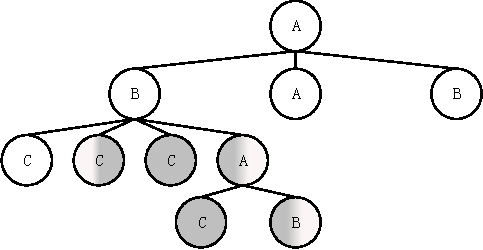
\includegraphics{partialtree/figures/fromWord-1.pdf}
\caption{An example XML tree}
\label{fig:example}
\end{figure}

\begin{figure}[t]
\centering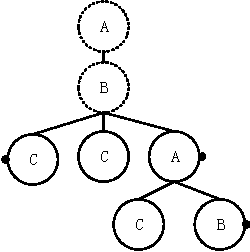
\includegraphics{partialtree/figures/fromWord-3.pdf}
\caption{Partial tree for the example.}
\label{fig:partialtree}
\end{figure}

In this paper, we deal with an important subset of XPath queries called
\emph{navigational XPath queries}~\cite{xpathcategory} in which we specify the nodes with not only
the parent-child relationships but also the inter-sibling relationships
and additional conditions called predicates.  Although a partial tree has
the parent-child relationships from the root, it lacks the information
required to process navigational XPath queries, a node may have only some
of its children, and some siblings may be on another partial tree.
Therefore, we develop a new algorithm for processing navigational XPath
queries over a set of partial trees with communication.
Our algorithm is easy to implement because it processes the steps in a query (including those in predicates) 
one by one and is efficient because we carefully analyzed the conditions to reduce the communication among partial trees.

The contributions of our study are summarized as follows.

\begin{itemize}
\item \textbf{Formalizing the structure for XML chunks}:
We first formalize the structure and properties of partial trees that are given from chunks of an XML document (Section~\ref{sec:partialtree}). We also show an algorithm to parse the chunks and construct the partial trees (Section~\ref{sec:construction}).

\item \textbf{Parallelizing XPath Queries}:
We then develop an algorithm for executing the navigational XPath queries in parallel (Section~5).
Basically, the algorithm runs independently on partial trees, but it also performs communication
to obtain the correct query results.

\item \textbf{Experiments on GB-level XML documents}:
We implemented the algorithm in Java and conducted experiments on a PC cluster with GB-level XML documents (Section~6).  Our implementation successfully processed an 8 GB XML document in parallel and obtained speedups of a factor of 6.0 over 16 PCs.
\end{itemize}


The remainder of the paper is organized as follows. In Section 2, we review the XPath query. In Section 3, we discuss the partial trees in detail. In Section 4, we discuss how to construct partial trees from chunks of an XML document. In Section 5, we discuss executing XPath query  algorithms in parallel. We 
report the experiment results in Section 6. Related work is shown in Section 7, and we conclude the paper in Section 8.


% LocalWords: kmatsu 
	% background information
% this file is called up by thesis.tex
% content in this file will be fed into the main document

\chapter{Aims of the project} % top level followed by section, subsection


% ----------------------- contents from here ------------------------

\section{Final aim}

Our ultimate goal is...

\section{Preliminary aims}

There will be several preliminary scientific targets to be accomplished on the way...




% ---------------------------------------------------------------------------
% ----------------------- end of thesis sub-document ------------------------
% ---------------------------------------------------------------------------						% aims of the project

\include{3/XYZ}			
\include{4/XYZ}	
\include{5/XYZ}
\include{6/XYZ}

% this file is called up by thesis.tex
% content in this file will be fed into the main document

\chapter{Discussion} % top level followed by section, subsection


% ----------------------- paths to graphics ------------------------

% change according to folder and file names
\ifpdf
    \graphicspath{{7/figures/PNG/}{7/figures/PDF/}{7/figures/}}
\else
    \graphicspath{{7/figures/EPS/}{7/figures/}}
\fi


% ----------------------- contents from here ------------------------






% ---------------------------------------------------------------------------
% ----------------------- end of thesis sub-document ------------------------
% ---------------------------------------------------------------------------               % discussion of results


% this file is called up by thesis.tex
% content in this file will be fed into the main document

\chapter{Materials \& methods} % top level followed by section, subsection


% ----------------------- paths to graphics ------------------------

% change according to folder and file names
\ifpdf
    \graphicspath{{8/figures/PNG/}{8/figures/PDF/}{8/figures/}}
\else
    \graphicspath{{8/figures/EPS/}{8/figures/}}
\fi

% ----------------------- contents from here ------------------------




 

% ---------------------------------------------------------------------------
%: ----------------------- end of thesis sub-document ------------------------
% ---------------------------------------------------------------------------



 






        % description of lab methods




% --------------------------------------------------------------
%:                  BACK MATTER: appendices, refs,..
% --------------------------------------------------------------

% the back matter: appendix and references close the thesis


%: ----------------------- bibliography ------------------------

% The section below defines how references are listed and formatted
% The default below is 2 columns, small font, complete author names.
% Entries are also linked back to the page number in the text and to external URL if provided in the BibTex file.

% PhDbiblio-url2 = names small caps, title bold & hyperlinked, link to page 
\begin{multicols}{2} % \begin{multicols}{ # columns}[ header text][ space]
\begin{tiny} % tiny(5) < scriptsize(7) < footnotesize(8) < small (9)

\bibliographystyle{Latex/Classes/PhDbiblio-url2} % Title is link if provided
\renewcommand{\bibname}{References} % changes the header; default: Bibliography

\bibliography{9_backmatter/references} % adjust this to fit your BibTex file

\end{tiny}
\end{multicols}

% --------------------------------------------------------------
% Various bibliography styles exit. Replace above style as desired.

% in-text refs: (1) (1; 2)
% ref list: alphabetical; author(s) in small caps; initials last name; page(s)
%\bibliographystyle{Latex/Classes/PhDbiblio-case} % title forced lower case
%\bibliographystyle{Latex/Classes/PhDbiblio-bold} % title as in bibtex but bold
%\bibliographystyle{Latex/Classes/PhDbiblio-url} % bold + www link if provided

%\bibliographystyle{Latex/Classes/jmb} % calls style file jmb.bst
% in-text refs: author (year) without brackets
% ref list: alphabetical; author(s) in normal font; last name, initials; page(s)

%\bibliographystyle{plainnat} % calls style file plainnat.bst
% in-text refs: author (year) without brackets
% (this works with package natbib)


% --------------------------------------------------------------

% according to Dresden med fac summary has to be at the end
%
% Thesis Abstract -----------------------------------------------------


%\begin{abstractslong}    %uncommenting this line, gives a different abstract heading
\begin{abstracts}        %this creates the heading for the abstract page

Put your abstract or summary here, if your university requires it.

\end{abstracts}
%\end{abstractlongs}


% ---------------------------------------------------------------------- 


%: Declaration of originality

% Thesis statement of originality -------------------------------------

% Depending on the regulations of your faculty you may need a declaration like the one below. This specific one is from the medical faculty of the university of Dresden.

\begin{declaration}        %this creates the heading for the declaration page

I herewith declare that I have produced this paper without the prohibited assistance of third parties and without making use of aids other than those specified; notions taken over directly or indirectly from other sources have been identified as such. This paper has not previously been presented in identical or similar form to any other German or foreign examination board.

The thesis work was conducted from XXX to YYY under the supervision of PI at ZZZ.

\vspace{10mm}

CITY,


\end{declaration}


% ----------------------------------------------------------------------



\end{document}
